\documentclass[../report.tex]{subfiles}

\begin{document}
\graphicspath{{img/}{../img/}}


\section{Gantt planl�gning}
Gantt er en udbyggelse af den klassiske tidsplan. Den er lavet for at give et bedre overblik over de forskellige planlagte opgaver i forhold til hinanden. Hvor en klassisk tidsplan i form af en tabel er fokuseret p� tidsperioderne, er et Gantt diagram fokuseret p� arbejdsopgaverne.\\

Figur~\ref{fig:Gantt} viser Gantt diagrammet for target projektet. Diagrammet er meget skrabet, da aktiviteter i den valgte procesmodel, Scrum(se afsnit \ref{sec:Scrum}), opdeles og estimeres l�bende. Gantt diagrammet er alts� lavet p� baggrund af en delvis nedbrydning af aktiviteter (se afsnit \ref{sec:Activity Breakdown} om activity breakdown), og et estimat ikke p� arbejdstimer, men et bud p� hvor stor en del af projektet en del-aktivitet kan tage. \\

Havde target projektet brugt en vandsfaldsmodel (se afsnit \ref{sec:Waterfall} om vandfaldsmodel) kunne man have valgt at lave et fuldt product og activity breakdown for s� at estimere det hele og lave Gantt diagrammet.
\\ \\


\begin{figure}[H]
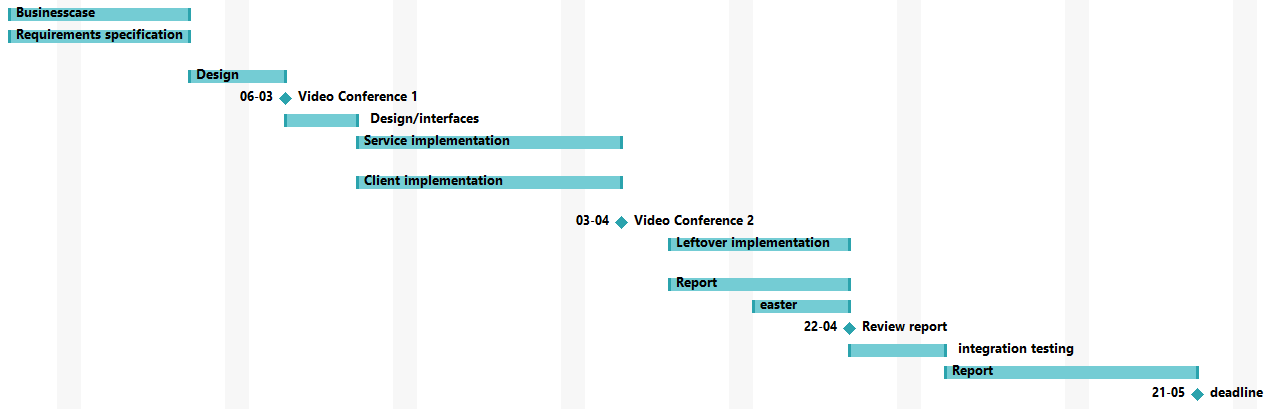
\includegraphics[scale=0.45]{TargetProjectGantt.png}
\caption{Gantt diagram for target projektet}
\label{fig:Gantt}
\end{figure}

Gantt diagrammet vinder stort inden for overblik mod den klassiske tidsplan, men i n�ste kapitel kigges der p� et andet alternativ til aktivitetsplanl�gning.



\end{document}